\chapter{State of the art}
\section{Noise Removal in Image Processing using Median}

This paper "Noise Removal in Image Processing using Median, Adaptive
Median and Proposed Median Filter and Respective Image
Quality Comparison" was written by Monika Kohli and Harmeet Kaur. Authors research and analyze median filter. From this, the filter is compared with median and Adaptive median filter. 
\vspace{1cm}

\textbf{Types of noise}
\begin{itemize}
\item Impulse noise (Salt \& pepper noise)
\item Amplifier noise (Gaussian noise)

\item Quantization noise (Uniform noise)

\item Multiplicative noise (Speckle noise) 
\item Periodic noise(Stationary noise)
\end{itemize}
\vspace{0.5cm}

After image noise can be classified as above, characteristics of each type are specified. Next to analyse algorithm of filters : Median filter, Adaptive median filter, Proposed Median Filter.  
\vspace{1cm}

\textbf{Result Comparison of filters:}

\

For: Salt and Pepper noise as 0.01 and 0.02 respectively. 
\vspace{1cm}

\begin{tabular}{|c|c|c|c|}
\hline 
 & Median Filter & Adaptive Median Filter & Proposed Median Filter \\ 
\hline 
LENA(0.01) & 27.85 & 28.62 & 29.17 \\ 
\hline 
LENA(0.02) & 26.92 & 27.37 & 27.65 \\ 
\hline 
\end{tabular} 
\vspace{1cm}

Finally, result Comparison of filters when used PSNR to calculate quality of images. We obtained result show that the proposed method is the best.In futher, result can be improved by different noise such as : Gaussian noise, Speckle noise etc


\section{The Sure-Let Approach to Image Denoising}

The paper was written by Thierry Blu, Senior Member, IEEE, and Florian Luisier. It's a new approach to image denoising,
based on the image-domain minimization of an estimate of the
mean squared error(MSE).


\begin{itemize}
\item A new approach to image denoising,based on the image-domain
minimization of an estimate of the mean squared error:
Stein’s unbiased risk estimate (SURE)
\item The denoising process can be expressed as a linear combination of
elementary denoising processes:
Linear expansion of thresholds (LET)
\item Evaluate this denoising performances by comparing PSNR
\item Combined 3 step above to  SURE-LET Approach
\end{itemize}

We have SURE-LET Formula as below :

\vspace{0.5cm}
$\displaystyle\sum_{l=1}^{K}\underbrace{F_k(y)^T F_l(y)a_l}_{[M]_{k,l}} = \underbrace{F_k(y)^Ty-\sigma^2div\left\{F_k(y)\right\}}_{[c]_k}$     
\vspace{0.2cm}

$$\hspace{-5cm} for \ k = 1,2...K$$	
\begin{center}
\hspace{-5cm} 	$\vspace{0.3cm}\Updownarrow$ 
	

\hspace{-5cm}	\textbf{Ma=c} 
\end{center}

\textbf{Result:}

\

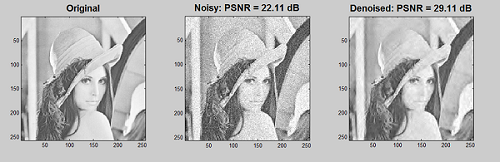
\includegraphics{surelet1.png}

\begin{itemize}
	\item Input PSNR   : 22.11[dB] 
	\item Output PSNR  : 29.11[dB]
	\item Elapsed time : 0.55[s]
\end{itemize}

With \textbf{$PSNR = 10*log_{10}(255^2/MSE)$}, we have :
\begin{itemize}
	\item Input PSNR   : 22.11[dB] \ $\Rightarrow$ Input MSE = 4.00
	\item Output PSNR  : 29.11[dB] \ $\Rightarrow$ Output MSE = 3.22
\end{itemize}
\textbf{Conclude:}

\

Follow SURE-LET program in Matlab, input MSE is compare between noisy image and original image, output MSE is compare between denoise image and original image. So we use output MSE result to table of Comparison Of The Results.

\section{Study on Methods of Noise Reduction in a Stripped Image}

Author's this paper: Chi Chang-yan, Zhang Ji-xian, Liu Zheng-jun

\

Noise is one of  image quality problem in the image processing major. Noise reduction is necessary for us to do remove noise and description useful information more prominent. The Gray Value Substitution and Wavelet Transformation are methods in noise removal. Finally, MSE and PSNR are evaluated the processed image suitable in this paper.


\subsection{Low pass filter}
\begin{center}
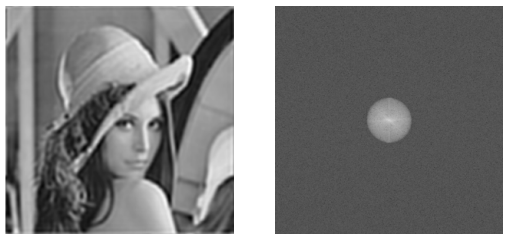
\includegraphics{lowpass.png}


TLPF processed image and its Fourier spectrum 
\end{center}
Noise is high frequency signal, so we used  low pass filter to reduce it. The trapezium low pass filter (TLPF) we choose has certain advantage to smooth transition band. After processing, the image is blur than that before. Low pass filter can remove noise is meaning detailed image information is also removed. So it is not good at image which needs much spectral information. 

\subsection{Gray Value Substitution }
\begin{center}
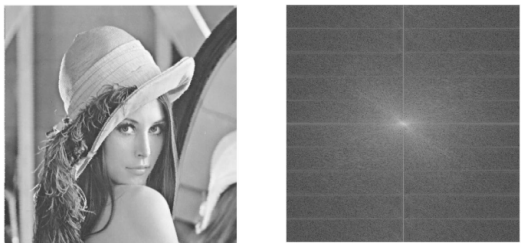
\includegraphics{gray.png}

 Image processing results of gray value substition 
\end{center}

We can see from this image, most noise line is changed and it is not affected by this method.  However, some small noise still appear, and the brightness after processing is stronger than that before. 

\subsection{Wavelet transformation }

\begin{center}
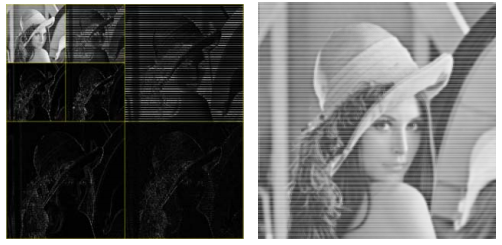
\includegraphics{wave.png}

Image decomposition using Wavelet and usual wavelet denoising result
\end{center}
Wavelet method  haven't solution remove noise which still exists in the horizontal domain, the vertical and cross part of this image does not have much noise. 

\subsection{Results and comparisons }
\vspace{1cm}

\begin{center}


\begin{tabular}{|c|c|c|}
\hline 
Noisy Image  & MSE & PSNR \\ 
\hline 
Low Pass Filter  & 1260.8 & 17.1242  \\ 
\hline 
Gray Value Substitution & 28.0140 & 33.6571  \\ 
\hline 
Wavelet transformation  & 8.8177  & 38.6773  \\ 
\hline 
\end{tabular} 

\

Results and comparisons of MSE and PSNR 
\end{center}

From result tables, we can see that, low pass filter can't use to remove noise. And the other two methods is relatively accepted

\section{Different Noise Types and Digital Image Processing}
(Gursharan Kaur, Rakesh Kumar, Kamaljeet Kainth)


As we know, image is used in various fields like medical and education.But noise is bad problem to image.So noise reduction is the main focus to retain the quality of the image.This paper is review problem to types of noise and solution.

\subsection{TYPES OF NOISE}
\begin{itemize}
\item Gaussian noise
\item Salt and pepper noise
\item Poisson noise
\end{itemize}

\subsection{DIFFERENT TYPES OF LINEAR AND NON-LINEAR FILTERS}
\begin{itemize}
\item Mean Filter: Mean filter is a type of linear filter that computes average value of the corrupted image.
\item Median Filter: Median filter is a type of non-linear filter. It used to reduce the amount of intensity variation between one pixel and the other pixel.
\end{itemize}

\subsection{CONCLUSION AND FUTURE SCOPE}
In this paper, different techniques are used to remove noise from the image.Techniques that are already using may not be able to find the best result so in the future we may find the techniques that provide optimum solution to the noise.


\section{Impulse Noise Reduction
methods in Digital images
}

"A comparative study of Impulse Noise Reduction methods in Digital images", Authors: Himani Goel, Seema Rani. As paper title, we'll review this paper about denoise. From this, compare results by PSNR and MSE to obtain best result. 

\subsection{Linear Filters}
\begin{itemize}
\item Mean filter
\item Wiener filter
\end{itemize}

\subsection{Non Linear filters}
\begin{itemize}
\item Adaptive median
filter
\item Improved progressive
switching median
filter
\end{itemize}

\subsection{Conclusion}
\begin{center}


\begin{tabular}{|c|c|c|}
\hline 
Filter Types & MSE & PSNR \\ 
\hline 
Mean filter & 169.52 & 25.12 \\ 
\hline 
Average filter & 169.52 & 25.12 \\ 
\hline 
Adaptive median
filter & 30.51 & 36.71 \\ 
\hline 
Improved progressive
switching median
filter & 196.36 & 37.32
 \\ 
\hline 
\end{tabular} 
\end{center}


By the results from table above, we see the median filtering is better than mean or average filter to remove impulse noise but it affect the edge details.


%This chapter must discuss about the different papers addressing the same topics of your internship.
%You must be able to explain the work published, by giving the context of the work, the main idea, the main results, and you must also be able to analyze the proposal.

\vspace*{2cm}



%You must cite the articles you have read. The citations must be done as follow. \\



\vspace*{2cm}

%In the paper \cite{Abr98}, the authors explain how ....

\vspace*{1cm}


%The work presented in  \cite{Hau03b} considers the problem of ...


\vspace*{1cm}

%In \cite{Ham95}, the results show that .....


\vspace*{1cm}

%In comparison with \cite{Hau03a}, the method is ...

